\documentclass{bioinfo}
\copyrightyear{2007}
\pubyear{2007}
%$Revision$
%$LastChangedDate$
%$Author$

\begin{document}
\firstpage{1}

\title[Discrete Stochastic Models Test Suite]{The SBML Discrete Stochastic Models Test Suite}
\author[Evans, T. W. \textit{et~al}]{Thomas W. Evans\,$^{1}$, Colin S. Gillespie\,$^{2,3}$ and Darren J. Wilkinson\,$^{2,3}$\footnote{to whom correspondence should be addressed}}
\address{$^{1}$Department of Mathematical Sciences, University of Liverpool, Liverpool, L69 7ZL.\\
$^{2}$School of Mathematics \& Statistics, Newcastle University,
Newcastle upon Tyne, NE1 7RU, UK.\\
$^{3}$Centre for Integrated Systems Biology of Ageing and Nutrition
(CISBAN), Newcastle University.}

\history{Received on ...}

\editor{Associate Editor: ...}

\maketitle

\begin{abstract}

\section{Motivation:}
Stochastic simulation is a very important tool for mathematical
modelling. However it is difficult to check the correctness of a
stochastic simulator, since any two realisations from a single model
will typically be different.

\section{Results:}
We have developed a test suite of stochastic models which have been solved either analytically or using numerical methods. This allows the accuracy of stochastic simulators to be tested against known results. The test suite is already being used by a number of stochastic simulator developers.

\section{Availability:}
The latest version of the test suite can be obtained from
http://www.calibayes.ncl.ac.uk/Resources/dsmts/ and is licensed under
GNU Lesser General Public License.

\section{Contact:} \href{d.j.wilkinson@ncl.ac.uk}{d.j.wilkinson@ncl.ac.uk}
\end{abstract}

\section{Introduction}

In recent years it has been increasingly recognised that mathematical
modelling can help us to understand complex biological networks. As a
result of this, the Systems Biology Markup Language (SBML) was
developed as a standard format in which to represent the models
\citep{Hucka03}. SBML is quickly becoming the lingua franca for the
development and sharing of biochemical network models.

One popular modelling technique is to use a discrete stochastic kinetic framework. However, testing the correctness of the implementation of the underlying algorithm is difficult, since a stochastic simulator will by definition give you a different realisation for each run (for a different seed). This is especially
problematic since it is possible for two exact algorithms, such as 
Gillespie's direct method \citep{Gillespie77} and the Next Reaction
Method \citep{GibsBruc00}, to have different implementations 
and to use random number streams in an entirely different way.

A further complication in establishing the correctness of a simulator
arises from issues of interpretation of the SBML model representation. 
The SBML specification contains little guidance relating to the proper 
procedures to be followed in encoding models intended for discrete 
stochastic simulation (though the latest specification does contain 
an example), leading to potential confusion. Indeed, SBML Level 1 
was not capable of encoding discrete stochastic kinetic models in a 
correct, accurate and unambiguous way. Fortunately SBML Level 2 
and beyond are quite capable in this regard. See the discussion in
Chapter 2 of \cite{Wilkinson06} for further details. 

This paper describes how the SBML discrete stochastic models test
suite (DSMTS) can be used to test a stochastic simulator. Versions of the test
suite exist for SBML Level~2, versions~1 and~3. 


\section{Testing a Stochastic Simulator}

The only practical testing method is to run the simulator a large
number of times and check that the distribution of outcomes is not
significantly different from the true underlying distribution.
This can only be tested in a probabilistic way. The test suite is a
set of SBML models each with time course data for the means and
standard deviations of the model species. Developers may use the suite
to check that their simulators produce results that are consistent
with the SBML standard. The test suite assumes that the simulator
produces output on a regular time grid. Of course, exact stochastic
simulators naturally produce output on a non-regular grid
corresponding to individual reaction events (see \cite{Wilkinson06}
for further details on stochastic simulators). However, this ``step
function'' output is easy to map onto a regular time-grid either
post-hoc, or during the simulation run itself.

In order to test the output from an exact stochastic simulator for a
given SBML model (e.g. \cite{Gillespie77}), $n$ independent simulation
runs of the simulator should be performed. For the statistical tests
to have reasonable power to detect subtle problems, $n$ should be set
to at least 10,000. The sample means and standard deviations of the
species amounts from the simulation runs at $t=0,1,\ldots,50$ can be
compared with the corresponding values in the test suite using the
statistical tests described below. Figure \ref{figure1} shows the mean
and standard deviation over time for an example model which includes an
event. By comparing the output of many simulations to the true value,
we can test the stochastic simulator.
\begin{figure}[!t]
\centerline{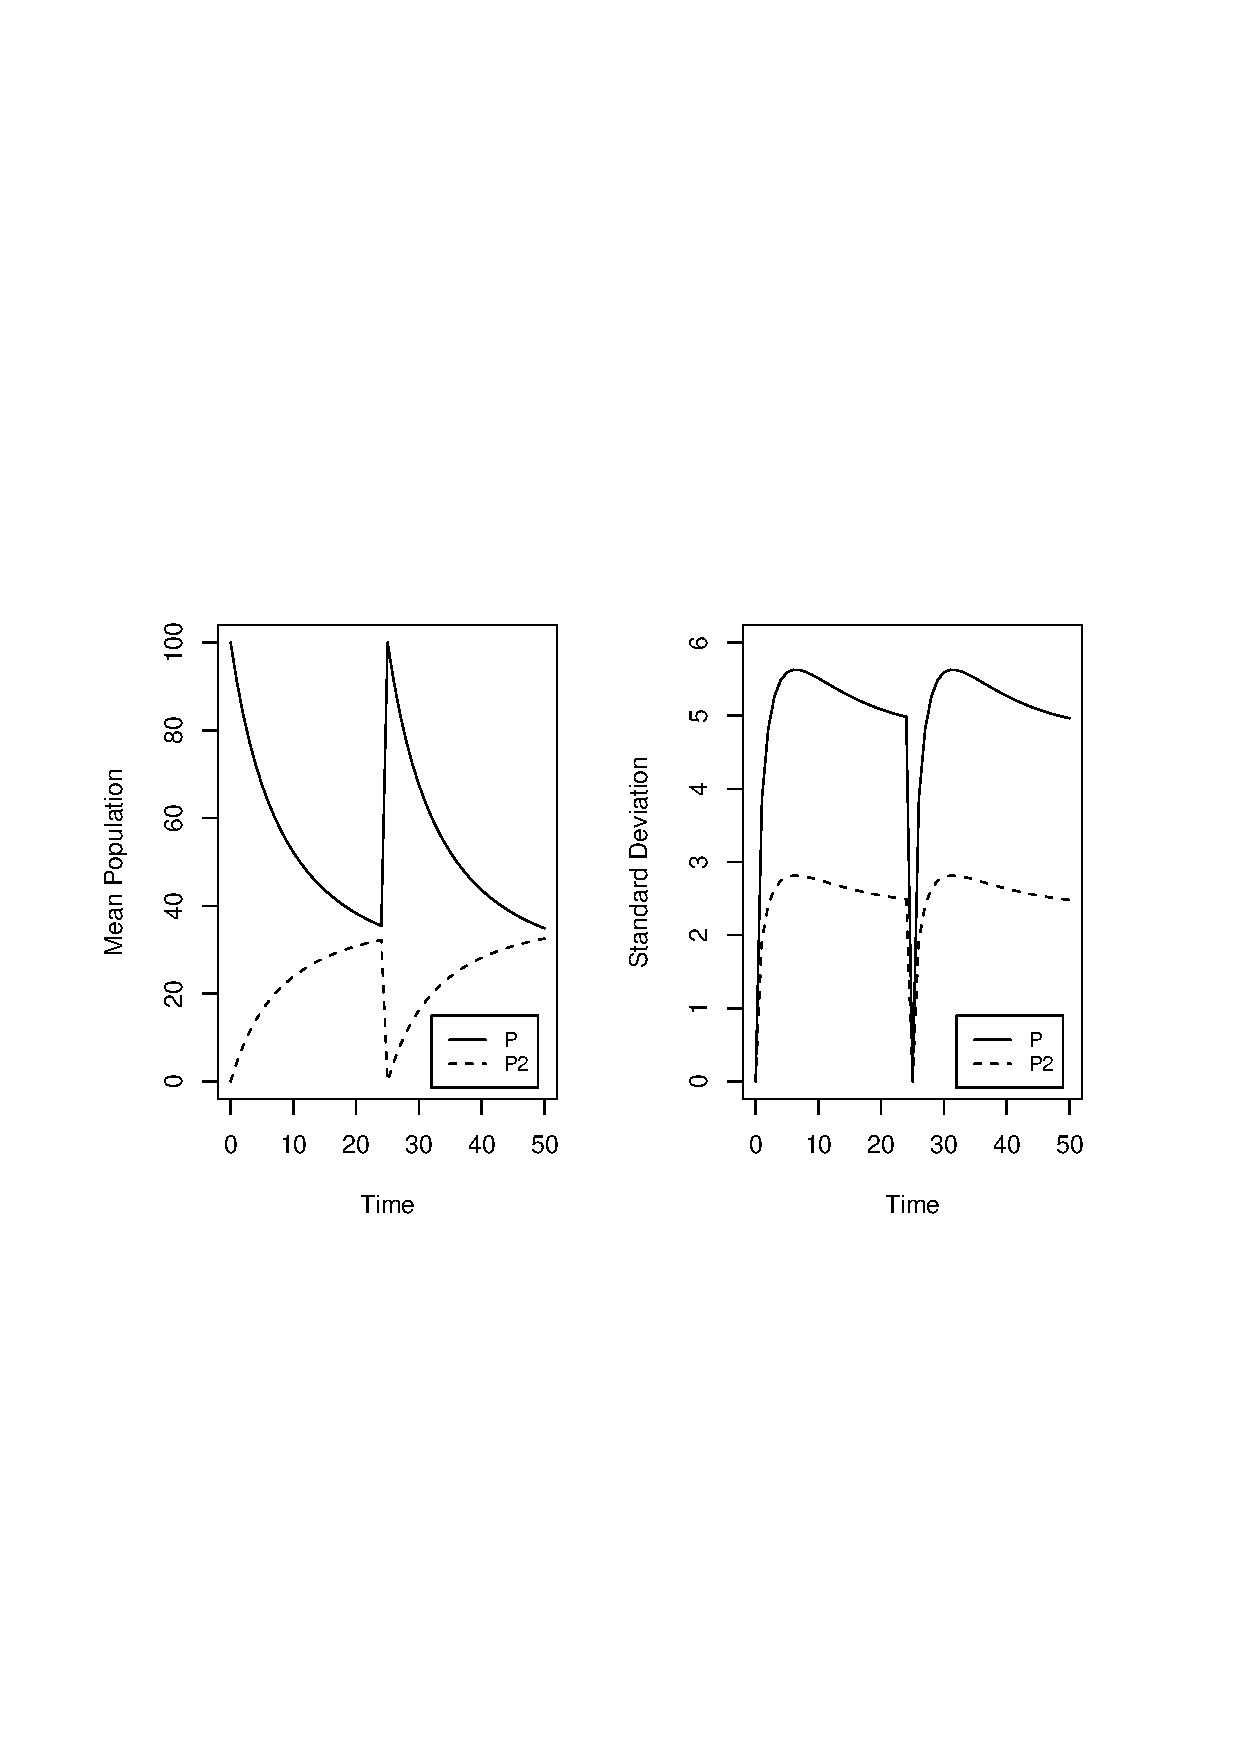
\includegraphics[scale=0.5,]{figure1.epsi}}
\caption{This figure represents a simple dimerisation model including SBML ``events''. When the time parameter $t$ becomes greater than or equal to 25, the species populations are reset to P = 100 and P2 = 0.}\label{figure1}
\end{figure}
The simulated values of a particular species, $X$, can be tested as
follows: let $X_t^{(i)}$ be the value of $X_t$ on the $i^{\mbox{th}}$
run of the simulator, where $X_t$ is the random variable representing
$X$ at time $t$. Put $\mu_t=\operatorname{E}(X_t)$ and
$\sigma_t=\sqrt{\operatorname{Var}(X_t)}$. Assuming that simulator
runs are independent, by the Central Limit
Theorem we have $$
\bar{X_t} \sim N( \mu_t, \sigma_t^2/n ),\ 
\text{ where }
\bar{X_t}=\frac{1}{n}\sum_{i=1}^n X_t^{(i)},
$$
giving
$$
Z_t \equiv \sqrt{n}\left( \frac{\bar{X_t} -\mu_t}{\sigma_t}\right)\sim N(0,1).
$$
So under the null hypothesis that the simulator is correct, the $Z_t$
values should have a standard normal distribution. In this case, most
values will lie in the range (-3,3). Therefore, values of $Z_t$
outside this range correspond to evidence that the simulator is in
error. The DSMTS User Guide also describes a test for the standard deviation.

Although the test suite is designed primarily for rigorous testing of exact simulators, it should also prove useful to developers of approximate simulators \citep{Gillespie03} or hybrid simulators \citep{Kiehl04, Puchalka04}. For example, one way of using the test suite to assess the performance of an approximate simulator is to plot the means and standard deviations as percentages of their true values.

The DSMTS currently uses variations of three simple models:
\begin{itemize}
\item The birth-death process (see \cite{Cox65} for details);
\item The dimerisation process \citep{Wilkinson06};
\item The batch immigration-death process, of which the classic immigration-death process is a special case \citep{Gillespie05}.
\end{itemize}
The models can be solved either analytically or, in the case of the
dimerisation model, by using numerical linear algebra. At
the time of writing there are 36 variations of the four models, and these
test a variety of SBML features, such as units, rate law
interpretation, events, and cell volumes. To run the entire test-suite takes approximately one hour, for $n=10,000$ and a reasonably fast simulator.

\section{Conclusion}

The test suite is already being employed by a number of stochastic
simulator developers. For example, the developers of the Systems
Biology Workbench
\citep{Hucka02,Vallabhajosyula07}, the BASIS system
\citep{Kirkwood03, Gillespie06} and COPASI \citep{Hoops06} all
use the test suite routinely. We have found the test suite to
be invaluable when developing our own stochastic simulator, as it provides
a simple and systematic means with which to test many aspects of the
simulator behaviour.

\section*{Funding}

Work on the DSMTS was partially funded by the BBSRC through grants
BEP 17042, BBS/B/16550, and BBC0082001.




\bibliographystyle{natbib}
\bibliography{refs}





\end{document}


